\section{Results \& Discussion}
\label{sec:result}
The result of gossip-based aggregation averaging simulation illustrated in section~\ref{sec:simulation} is visualised using R and shown in figure~\ref{fig:sim_result}. If we define $Converged$ as the state of every node is within 5\% of true value, which is mean value in our case. Let $\delta$ denote the smallest epoch number where this status is achieved, then a smaller value of $\delta$ implies better performance of a certain topology. Moreover, $\delta$ can be also seen as an attribute of convergence time $t$ as in our hypothesis.
\begin{figure}[h!]
	\centering
    \begin{subfigure}[t]{0.47\textwidth}
    \vspace{0pt}
    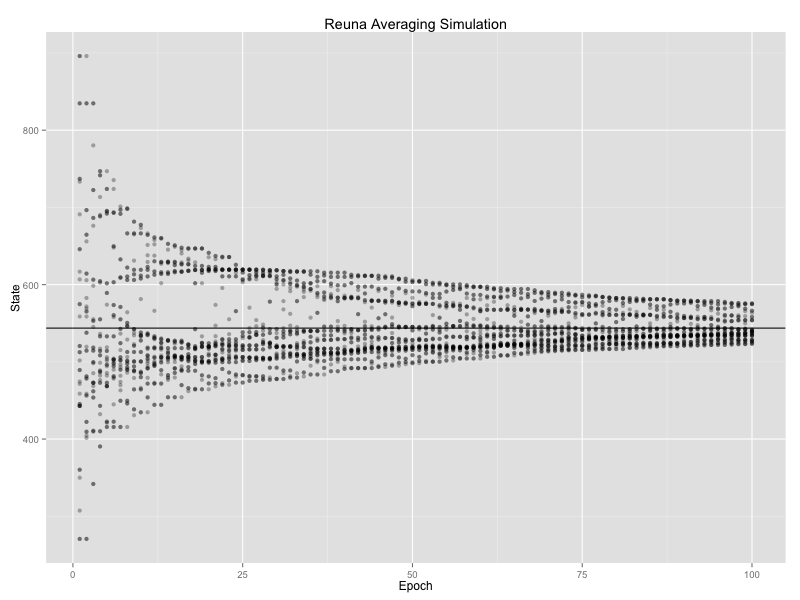
\includegraphics[width=\linewidth]{figures/Simulation_averaging/ReunaAvgSim.png}
    \caption{Reuna Averaging Simulation}
    \end{subfigure}
    %\vspace{5ex}
    \begin{subfigure}[t]{0.47\textwidth}
    \vspace{0pt}
    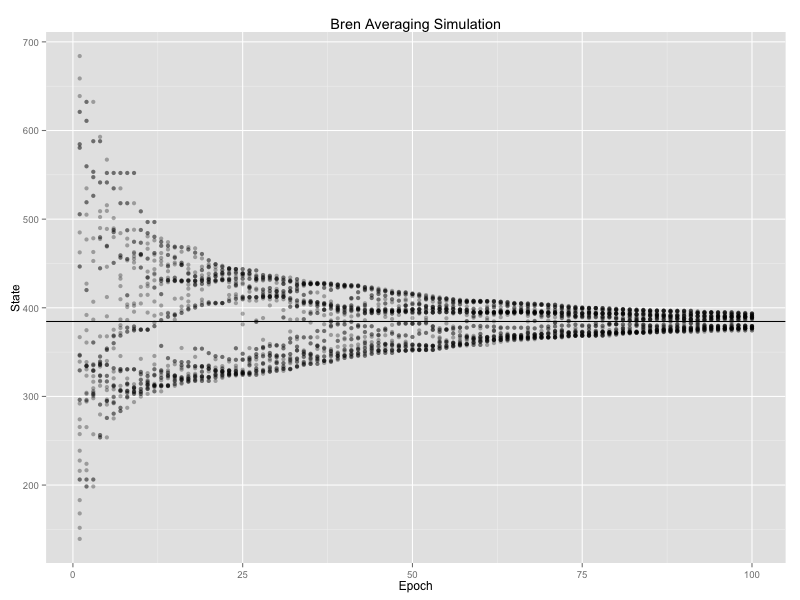
\includegraphics[width=\linewidth]{figures/Simulation_averaging/BrenAvgSim.png}
    \caption{Bren Averaging Simulation}
    \end{subfigure}
    \vspace{5ex}
    \begin{subfigure}[t]{0.47\textwidth}
    \vspace{0pt}
    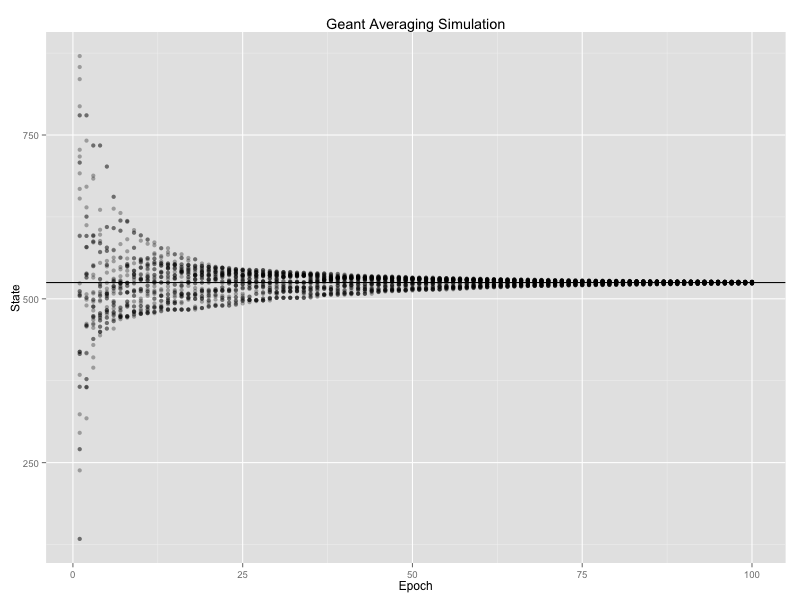
\includegraphics[width=\linewidth]{figures/Simulation_averaging/GeantAvgSim.png}
    \caption{Geant Averaging experiment}
    \end{subfigure}
    %\vspace{5ex}
    \begin{subfigure}[t]{0.47\textwidth}
    \vspace{0pt}
    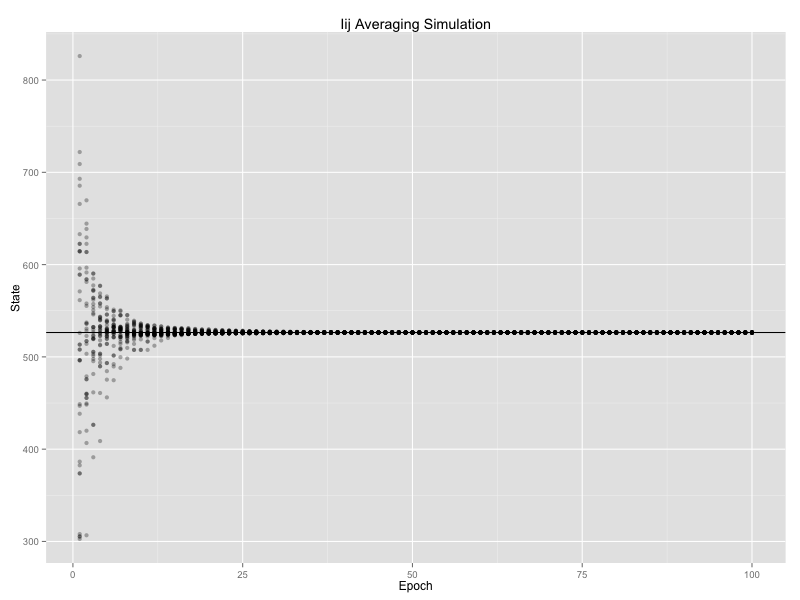
\includegraphics[width=\linewidth]{figures/Simulation_averaging/IijAvgSim.png}
    \caption{Iij averaging experiment}
    \end{subfigure}
    \caption{State changes of all nodes per epoch}
    \label{fig:sim_result}
\end{figure}
%TODO: define convergence criteria and derive the convergence speed.
Following this criteria, we can compute $\delta$ of each topology as shown in table~\ref{table:conv_epoch}. We can conclude from the table that the network with a higher number of links will gain a better performance in terms of convergence speed. Thus, the result of simulation supports our hypothesis. To be noticed that simulation of {\it Reuna} does not converge inside 100 epochs.
\begin{table}
\centering
\caption{Convergence epoch $\delta$ of each topology derived from simulation results}
\begin{tabular}{llc}
	\hline
	Name of Network &  \# of Links & $\delta$ \\
    	\hline
    	Reuna & 36 & NA\\
    	BREN & 38 & 98\\
    	Geant & 58 & 56\\
    	Iij & 66 & 18\\
    	\hline
\end{tabular}
\label{table:conv_epoch}
\end{table}

% aggregation of a random value from 0 to 1000
The results of our experiments are visualized in figure \ref{fig:result}. The X-axis are the epoch (time intervals) and the Y-axis is the state value. The gossip-based aggregation was run over 100 epochs. Every node started with a value chosen randomly between 0 and 1000. Due to the random nature of the algorithm and the difference in degree of connectivity among nodes a node can have between 1 and N state changes per epoch. (Where N is the amount of nodes in the network.) Overall nodes the number of state changes is 2*N per epoch. (Every node initiates one exchange per epoch which entails two state changes.) All of these changes are depicted.
\begin{figure}[h!]
	\centering
    \begin{subfigure}[t]{0.47\textwidth}
    \vspace{0pt}
    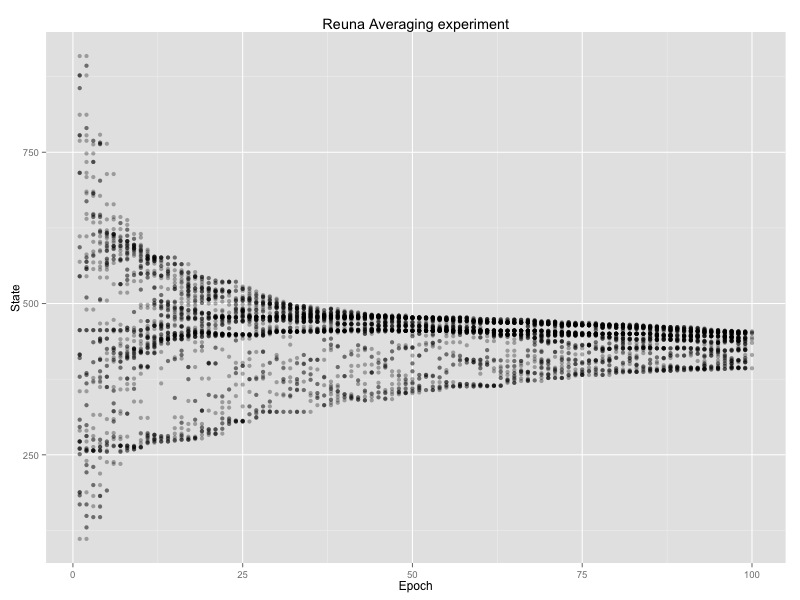
\includegraphics[width=\linewidth]{figures/Reuna.png}
    \caption{Reuna Averaging experiment}
    \end{subfigure}
    %\vspace{5ex}
    \begin{subfigure}[t]{0.47\textwidth}
    \vspace{0pt}
    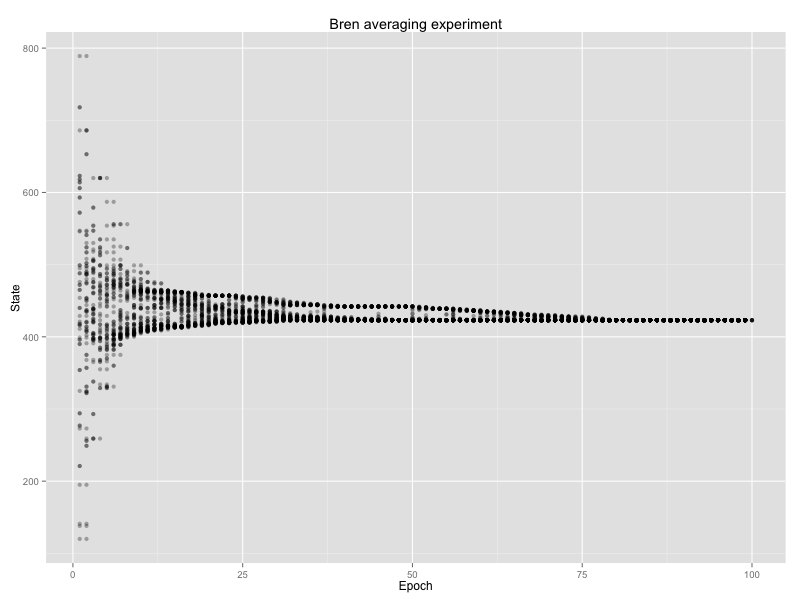
\includegraphics[width=\linewidth]{figures/Bren.png}
    \caption{Bren Averaging experiment}
    \end{subfigure}
    \vspace{5ex}
    \begin{subfigure}[t]{0.47\textwidth}
    \vspace{0pt}
    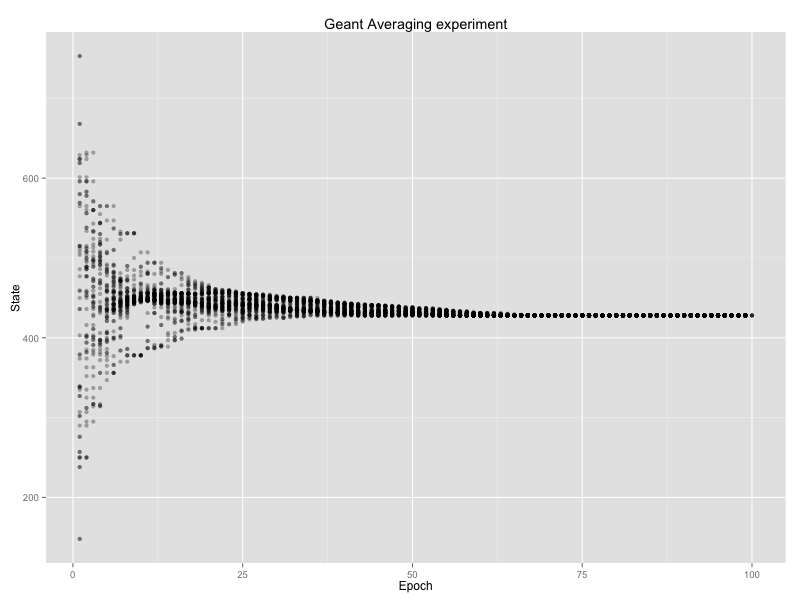
\includegraphics[width=\linewidth]{figures/Geant.png}
    \caption{Geant Averaging experiment}
    \end{subfigure}
    %\vspace{5ex}
    \begin{subfigure}[t]{0.47\textwidth}
    \vspace{0pt}
    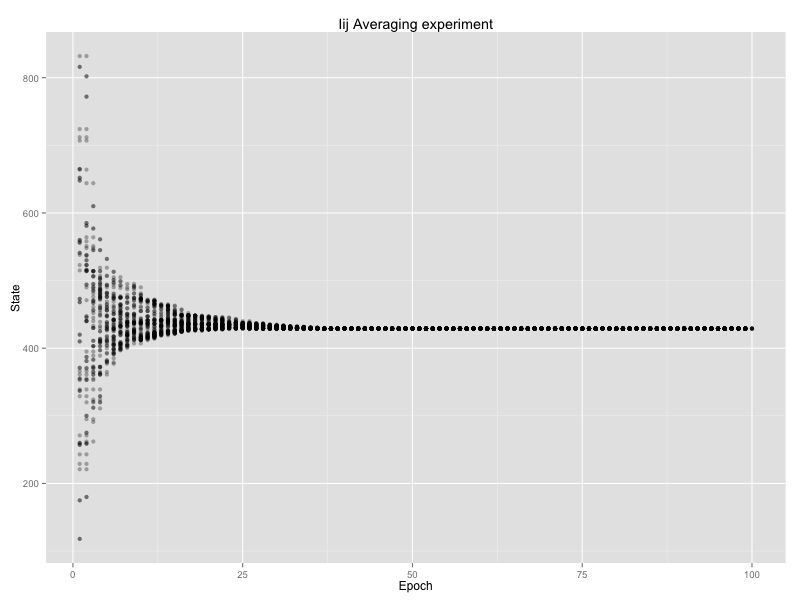
\includegraphics[width=\linewidth]{figures/Iij.png}
    \caption{Iij averaging experiment}
    \end{subfigure}
    \caption{State changes of all nodes per epoch}
    \label{fig:result}
\end{figure}
The graphs are sorted according to number of links per nodes from left to right and top to bottom. Inside 100 epochs all four experiments are in the trend of converging and if we set the same criteria as we analyse the result of simulation, $\delta$ of Bren, Geant and Iij could be derived as shown in table~\ref{table:exp}. Reuna does not converge inside the 100 epochs of our experiment.
\begin{table}
\centering
\caption{Convergence epoch $\delta$ of each topology derived from experiment results}
\begin{tabular}{llc}
	\hline
	Name of Network &  \# of Links & $\delta$ \\
    	\hline
    	Reuna & 36 & NA\\
    	BREN & 38 & 68\\
    	Geant & 58 & 52\\
    	Iij & 66 & 27\\
    	\hline
\end{tabular}
\label{table:exp}
\end{table}

Thus, the order of convergence speed can be derived as Iij, Geant, Bren, Reuna, from the fastest to slowest, which supports our hypothesis.
